%==============================================================================
%==============================================================================
\chapter{Displaying a Mesh}
\label{chap:display}

This chapter is on getting started with \GigaMesh\!. 
You may also go to chapter \ref{example} for brief examples in case you are already familiar with the program. 
Chapter \ref{detdia} gives a survey on the pulldown menu.
Keyboard shortcuts are summarized in the appendix \ref{keyboard}.

%==============================================================================
\section{First steps}

Open a console or a terminal and change into your \GigaMesh folder (with the {\tt cd GigaMesh} command). 
Then type {\tt ./gigamesh} and hit \Return\!.
\GigaMesh can be started using a file browser or from a menu entry, 
but it is recommended to be exectued within a terminal due to the output of additional information.
\begin{figure}[H]
	\begin{center}
		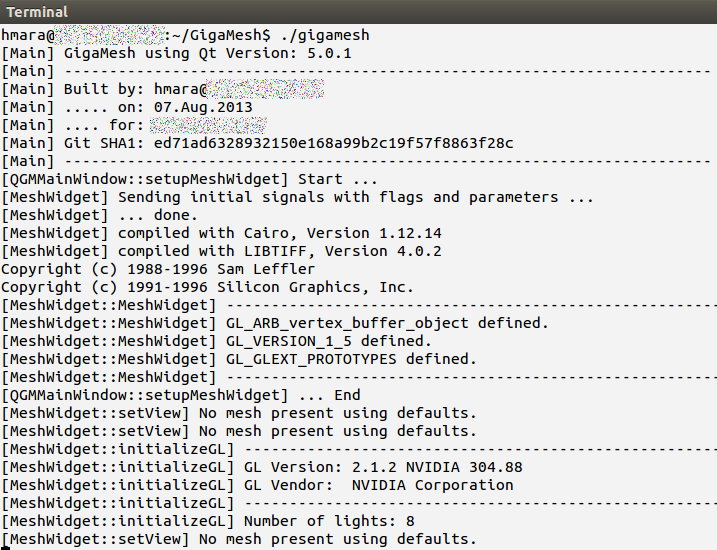
\includegraphics[height=64mm]{figs/gigamesh_console_output} 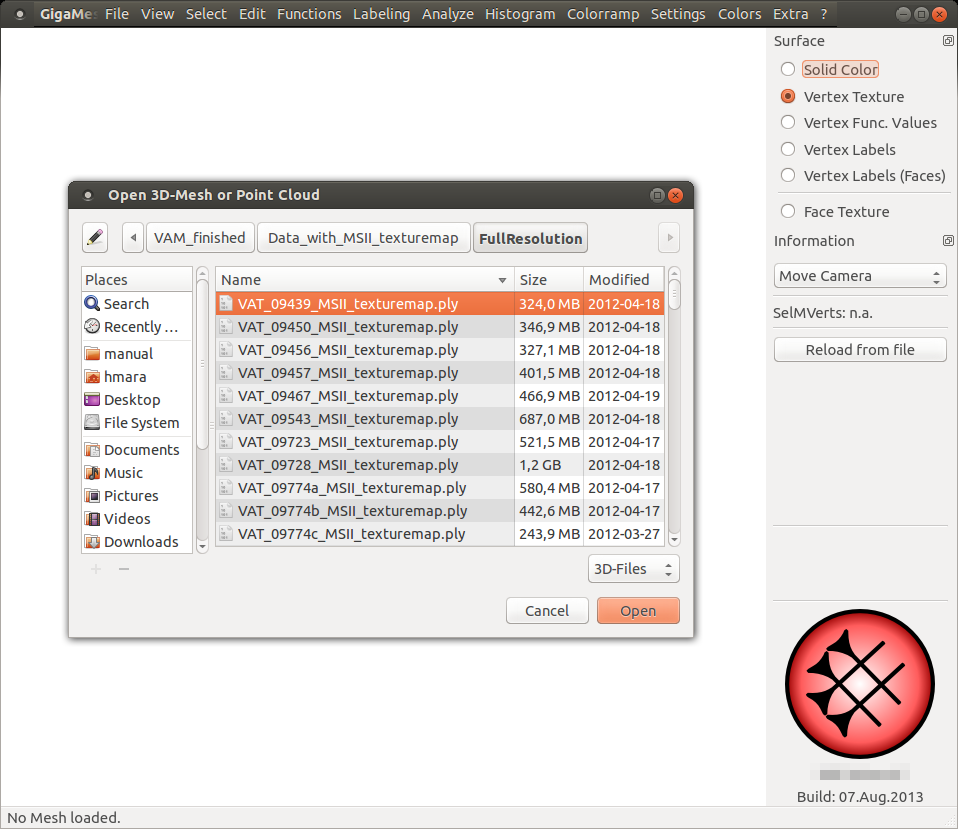
\includegraphics[height=64mm]{figs/gigamesh_gui_startup}
		\caption{Terminal in which you started \GigaMesh (left) and the graphical interface with the open file dialog (right).}\label{fig_start2}
	\end{center}
\end{figure}
As long as \GigaMesh is running it writes to the standard output device, i.e.~the terminal from which you started the program. 
So do not close this terminal, since all information concerning the current status of the program are displayed there. 
The program starts with the open file dialog window (see figure \ref{fig_start2}), where you can select the file you want to display and modify. 
A file browser and appropriate filter masks only show folders and 3D data with filename extensions PLY, OBJ, TXT, or XYZ.

After having opened a data file, the browser window disappears and the 3D object is displayed in the graphics window. 
Due to usually large data files of several hundreds of megabytes even reading the data may take some time (up to minutes). 
However, transformations work in realtime.

The graphics window has pulldown menu in the top bar and a sidebar with some buttons in top and the \GigaMesh logo at the bottom. 
Sketches to guide the user and a progress bar also appear in the sidebar. 
With the buttons in top the vertices change their colors from those given in the data file to no color at all or to the values given by some function value computed during the scope of the program and visualized with a certain color map.
For any task that might take some time, there is a progress bar above the logo and the \GigaMesh logo pops up in green (like a traffic light) for some seconds to signalize that the program is ready for the next commands.

\paragraph{Hint:} \GigaMesh can be started from the console with one given filename (no wildcards):
\begin{center}
	{\tt ./gigamesh [filename]} 
\end{center}

\newpage
%==============================================================================
\section{Viewing an Object}
\label{sec:viewing}

Generally the view can be changed using the move, the keyboard and by entering rotation angles.
Figure~\ref{fig:keyboardmove} show the keys used to navigate the OpenGL camera about an object.
The upper and middle row of keys change one of the three axis of the camera orientation by $1^\circ$.
With the lower keys the view can be changed by $90^\circ$, which allow a quick inspection of all side, top and bottom views.
\begin{figure}[!hbt]
	\centering
	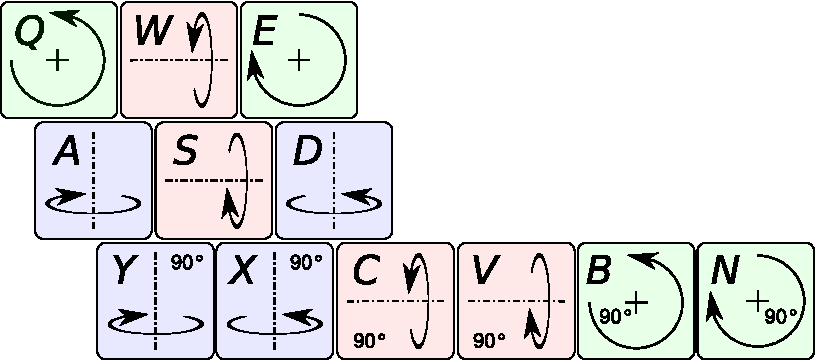
\includegraphics[height=50mm]{figs/gigamesh_keyboard_move_camera} % see GigaMesh/forms directory for the SVG source!
	\caption{Keyboard layout for navigating the OpenGL camera.}
	\label{fig:keyboardmove}
\end{figure}
The above Figure can also be (de-)activated within \GigaMesh using
\begin{itemize}
	\item[] \texttt{\fbox{?} $\rightarrow$ Keyboard Layout}.
\end{itemize}
Additional shortcuts are shown with
\begin{itemize}
	\item[] \texttt{\fbox{?} $\rightarrow$ Keyboard Shortcuts}.
\end{itemize}
In case a rotation about a specific angle e.g.~less than $1^\circ$ is required, the menus
\begin{itemize}
	\item[] \fbox{View}
	\begin{itemize}
		\item[$\rightarrow$] \texttt{Rotate Yaw (U/D)}, 
		\item[$\rightarrow$] \texttt{Rotate Pitch (L/R)} and
		\item[$\rightarrow$] \texttt{Rotate Roll}
	\end{itemize}
\end{itemize}
will provide a dialog to input an arbitrary value. 
The terms \emph{yaw}, \emph{pitch} and \emph{roll} refer to three critical flight dynamics parameters,
which are the angles of rotation about a vehicle's center of mass i.e.~the OpenGL camera's center.

\newpage
%==============================================================================
\section{Lighting}
\label{sec:lighting}

For lighting the object there are two lights available, one is enabled by default and can be switched on and off with \!\keystroke{1}\!. 
This light position and orientation is fixed to the view position and orientation -- in OpenGL terms: it is fixed to the camera.
The second light can be toggled \!\keystroke{2}\! and is fixed to the object and therefore does not move, when the view direction is changed.
The ambient light is enabled by default and can be toggled with~\!\keystroke{9}\!.
The amount of ambient light can be set by choosing the pulldown-menu
\begin{itemize}
	\item[] \texttt{\fbox{Settings} $\rightarrow$ Light Ambient -- Set Amount}.
\end{itemize}
You can turn on and off all lights together with the cutout switch for lighting which is assigned to \!\keystroke{0}\!.

Both virtual light sources project ideal parallel light.
Therefore only there orientation can be changed.
To change the orientation selected the according item from the Combo-Box on the right hand side:
\begin{figure}[!hbt]
	\centering
	\subfloat[]{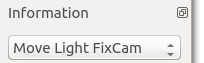
\includegraphics[keepaspectratio,width=0.4\textwidth]{figs/gigamesh_gui_move_light_fixedcam}\label{subfig:mousemodelightsA}} \quad
	\subfloat[]{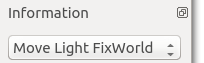
\includegraphics[keepaspectratio,width=0.4\textwidth]{figs/gigamesh_gui_move_light_fixedworld}\label{subfig:mousemodelightsB}}
	\caption{ Combo-Box choices for using the mouse to move the two lights with 
	          (a) fixed orientation to the camera and with 
	          (b) fixed orientation to the object.
	}
	\label{fig:mousemodelights}
\end{figure}

\paragraph{Hint:} The mode for manipulating the light orientation can be activated by short pressing\footnote{Holding \!\Alt and moving the mouse will move the window in \emph{Ubuntu Unity}.} 
the \!\Alt key for the first light.
To change the orientation of the second light, the \!\AltGr key has to be pressed while the mouse is moved.
To return to the default mode -- moving the view with the mouse -- the \!\Spacebar bar has to be pressed.
This will also change the Combo-Box to \texttt{Move Camera} as shown left in Figure~\ref{subfig:mousemodecamselA}.

\newpage
%==============================================================================
\section{Selection and Visualizing distances}
\label{distances}

The previous section showed the manipulation of the view and the light sources using mouse movement.
For selection there is an additional mode, 
which can either be selected from the Combo-Box or activated by holding the \!\Ctrl key.
In both cases the Combo-Box will show the term {\tt Selection} as shown in Figure~\ref{subfig:mousemodecamselA}.
Using the \!\Spacebar will return the operating mode of the mouse to manipulation of the view shown in Figure~\ref{subfig:mousemodecamselB}.
\begin{figure}[!hbt]
	\centering
	\subfloat[]{
\includegraphics[keepaspectratio,width=0.4\textwidth]{figs/gigamesh_gui_move_selection}\label{subfig:mousemodecamselA}} \quad
	\subfloat[]{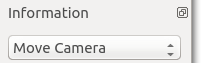
\includegraphics[keepaspectratio,width=0.4\textwidth]{figs/gigamesh_gui_move_camera}\label{subfig:mousemodecamselB}}
	\caption{ Combo-Box choices for using the mouse for
	          (a) interactive selection and
	          (b) to move the view direction (default).
	}
	\label{fig:mousemodecamsel}
\end{figure}

\vspace{-5mm}
\paragraph{Distance to a single vertex ({\tt SelVert}):}
The default selection allows to chose a single vertex. 
It can also be activated by
\begin{itemize}
	\item[] \texttt{\fbox{Select} $\rightarrow$ Primitive - Vertex SelVert/SelPrim}.
\end{itemize}
Therefore holding \!\Ctrl and single clicking with the left mouse button will select an appropriate vertex of the object. 
Then select {\tt Functions $\rightarrow$ Distance to SelPrim}. 
\begin{itemize}
	\item[] \texttt{\fbox{Functions} $\rightarrow$ Distance to SelPrim (COG)}.
\end{itemize}
All vertices get colored according to the default color map which is called {\tt Hot} and goes from black at the minimum over red to orange and finally white for the maximum. 
An overview of all possible color maps can be found in section \ref{color}.

\vspace{-5mm}
\paragraph{Distance to a plane:}
You may also measure the distances to a selected plane. 
Therefore change the selection mode to
\begin{itemize}
	\item[] \texttt{\fbox{Select} $\rightarrow$ Plane - 3 Points}
\end{itemize}
and note that a user guiding sketch of a triangle appears in the sidebar, when  \!\Ctrl is pressed. 
Select the three face points of the desired plane by single clicking on three vertices of the object. 
As long as this selection is active, you can change the position of the plane by clicking on other points of the object. 
You iteratively change the positions of the three defining face points. 
When you are satisfied with the selected plane chose
\begin{itemize}
	\item[] \texttt{\fbox{Functions} $\rightarrow$ Distance to Plane}
\end{itemize}
to displays the distance in shades of the current color map.

Figure~\ref{fig:distanceexamples} shows examples for distance to a single vertex and a plane, which are shown with and without lighting.
\begin{figure}[!hbt]
	\centering
	\subfloat[]{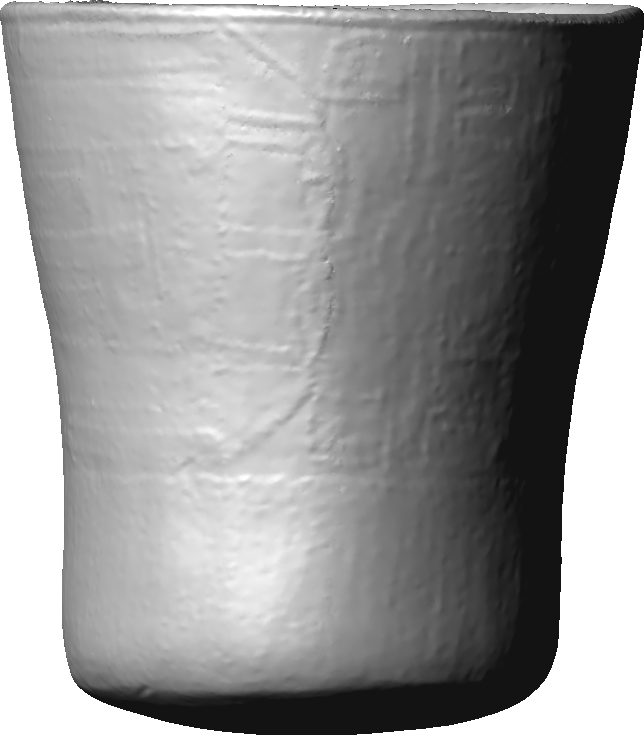
\includegraphics[keepaspectratio,width=0.3\textwidth]{figs/Nasca_Gefaess_GMOC_LightSolid}\label{subfig:distanceexamplesA}} \quad
	\subfloat[]{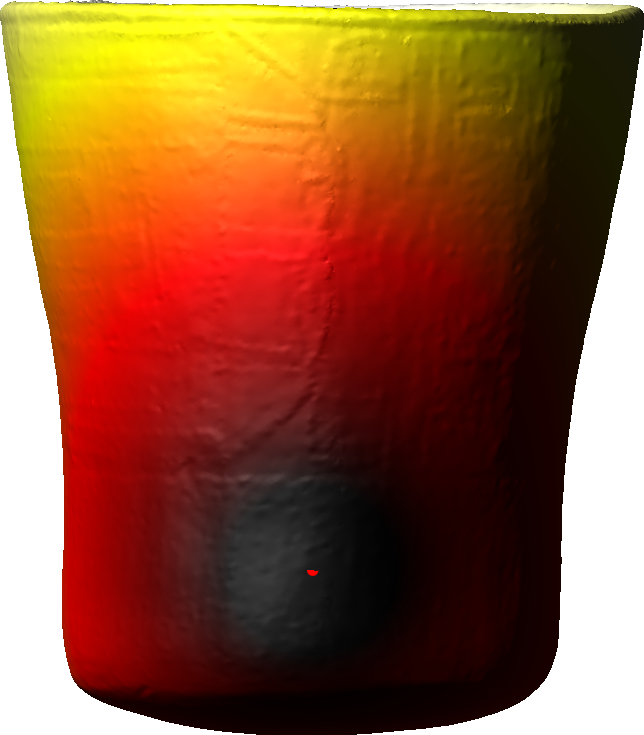
\includegraphics[keepaspectratio,width=0.3\textwidth]{figs/Nasca_Gefaess_GMOC_DistToVert_Light}\label{subfig:distanceexamplesB}} \quad
	\subfloat[]{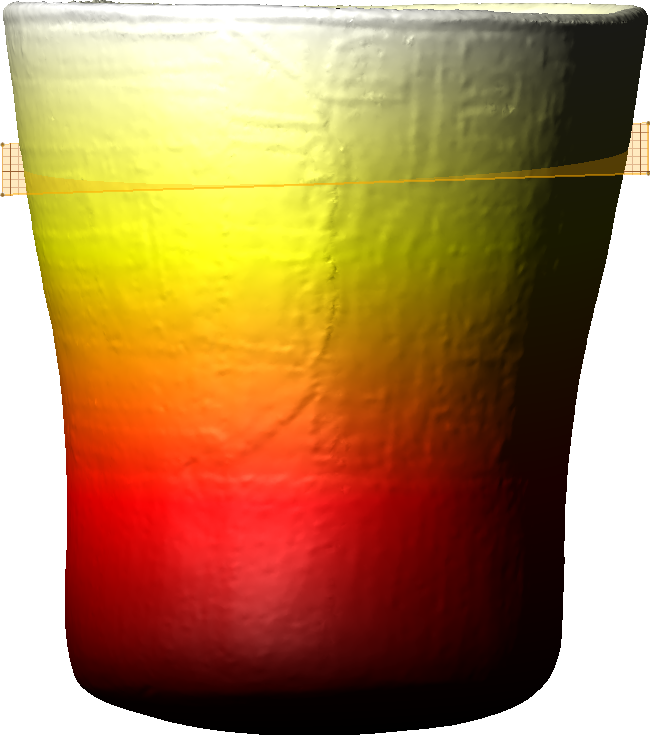
\includegraphics[keepaspectratio,width=0.3\textwidth]{figs/Nasca_Gefaess_GMOC_DistToPlane_Light}\label{subfig:distanceexamplesC}} \\
	\subfloat[]{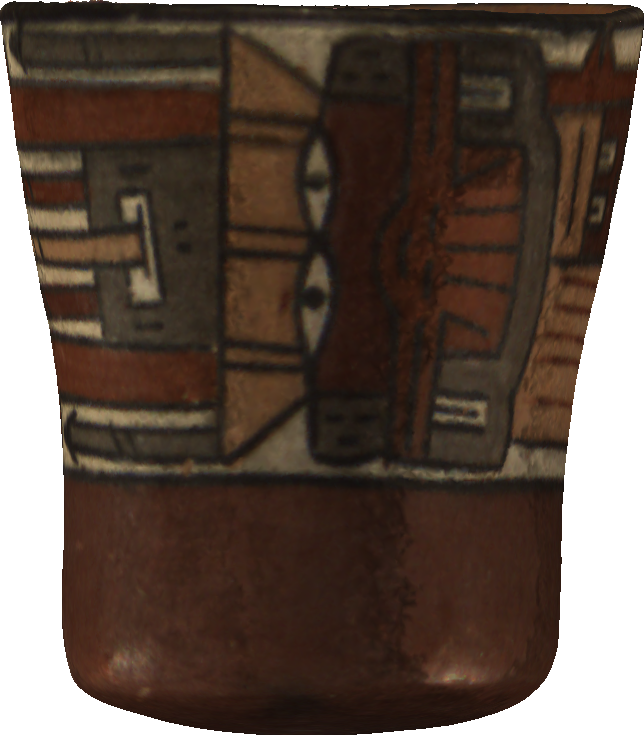
\includegraphics[keepaspectratio,width=0.3\textwidth]{figs/Nasca_Gefaess_GMOC_TexColor}\label{subfig:distanceexamplesD}} \quad
	\subfloat[]{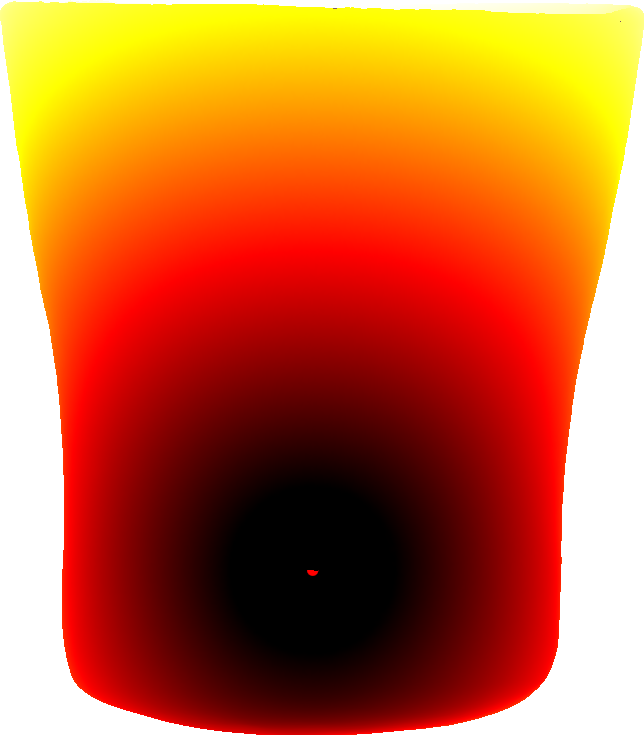
\includegraphics[keepaspectratio,width=0.3\textwidth]{figs/Nasca_Gefaess_GMOC_DistToVert}\label{subfig:distanceexamplesE}} \quad
	\subfloat[]{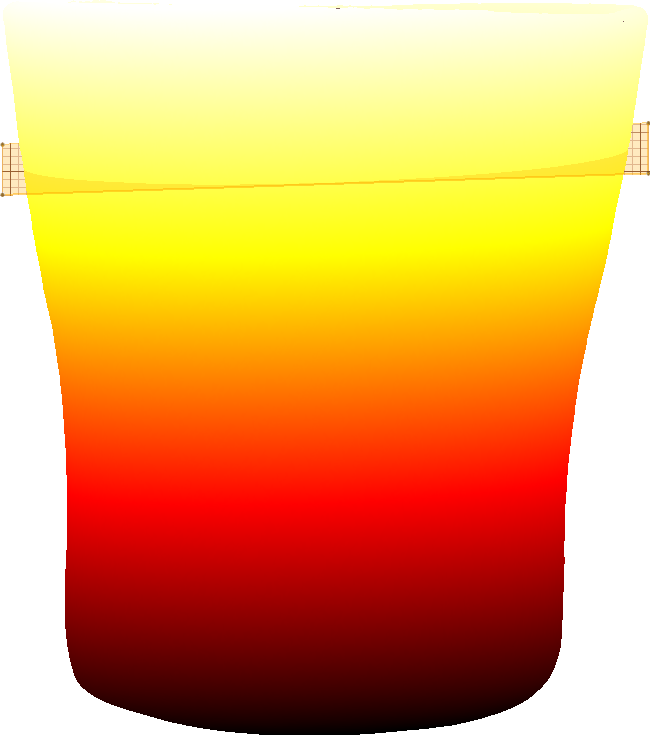
\includegraphics[keepaspectratio,width=0.3\textwidth]{figs/Nasca_Gefaess_GMOC_DistToPlane}\label{subfig:distanceexamplesF}} \\
	\caption{ Example for distance visualization on a replica of a (a,d) Nasca vessel. Distances to
	          (b,e) a single vertex ({\tt SelVert}) shown as red dot and
	          (c,f) to a plane shown in light orange color.
	          Light colors mean high values and dark colors mean low values.
	}
	\label{fig:distanceexamples}
\end{figure}

\clearpage
%==============================================================================
\section{Storing and Restoring the Default View}
\label{sec:defaultviewset}

The key \!\keystroke{F6} saves the current view of a 3D model to the default view.
This view and the default light positions can be retrieved by \!\keystroke{F12}\!. Pressing \!\Shift together with \!\keystroke{F12} also resets the zoom factor.
\begin{figure}[!hbt]
	\centering
	%\subfloat[]{}
	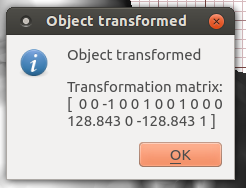
\includegraphics[height=50mm]{figs/gigamesh_gui_object_transformed}
%	\subfloat[]{ 
%	$
%		\left( %\fontsize{9}{9}\selectfont
%		\begin{array}{cccc} 
%			u/\sqrt{u^2+v^2}  & v/\sqrt{u^2+v^2} & 0 & 0 \\[1.5mm]
%			-v/\sqrt{u^2+v^2} & u/\sqrt{u^2+v^2} & 0 & 0 \\[1.5mm]
%			0 & 0 & 1 & 0 \\[1.5mm]
%			0 & 0 & 0 & 1
%		\end{array} \right)
%	 $
%	}
	\caption{Information window after setting the current view as default view.}
	\label{fig:objecttransformed}
\end{figure}
%[  0 0 -1 0 0 1 0 0 1 0 0 0 128.843 0 -128.843 1 ]
% rotation 90° vertical axis

\paragraph{Note:} As changing the default view is actually a change of position of the 3D model in world coordinates, 
the 3D model has to be saved to make the new default view permanent. 

\paragraph{Tip:} The transformation matrix shown in Figure~\ref{fig:objecttransformed} can be selected, copied and then saved as text-file. 
This allows to (re-)apply the same transformation later or to other 3D-models e.g.~when a new version of 3D-model was created from raw data.
The $16$ elements of the $4\times4$ matrix can be entered using the pulldown-menu
\begin{itemize}
	\item[] \texttt{\fbox{Edit} $\rightarrow$ Apply 4x4 Matrix -- All Vertices}.
\end{itemize}

%==============================================================================
\section{Meta-data}
\label{sec:metadata}

The model ID and its material get saved in the comment section of the header of the output file (e.g.~{\tt *.ply}). 
Note that this info gets lost when saving the file with external programs like e.g.~{\tt Meshlab}.
\GigaMesh asks to enter the meta-data, when a 3D-model is saved and no data is present.
It can also be edited selecting
\begin{itemize}
	\item[] \texttt{\fbox{Extra} $\rightarrow$ Cuneiform Figure Latex Info}
\end{itemize}
from the pulldown-menu. 
As the name indicates this functionality was introduced, when large amounts of cuneiform tablets were processed in the early days of \GigaMesh.
Therefore an additional \LaTeX{} template exists to easily prepare a corpus of 3D-models visualized with virtual illumination and MSII-based texture maps.

